\chapter{Processo de alinhamento}
\label{cap:processo}
Neste capítulo, será apresentado o processo proposto para alinhar dados. Como exibido na Figura \ref{fig:processo}, o processo é composto por 4 etapas principais, sendo elas: selecionar \textit{datasets}, identificar conceitos, listar recursos e alinhar dados. cada etapa do processo será descrita nas subseções a seguir.


\begin{figure}[!ht]
	\centering
	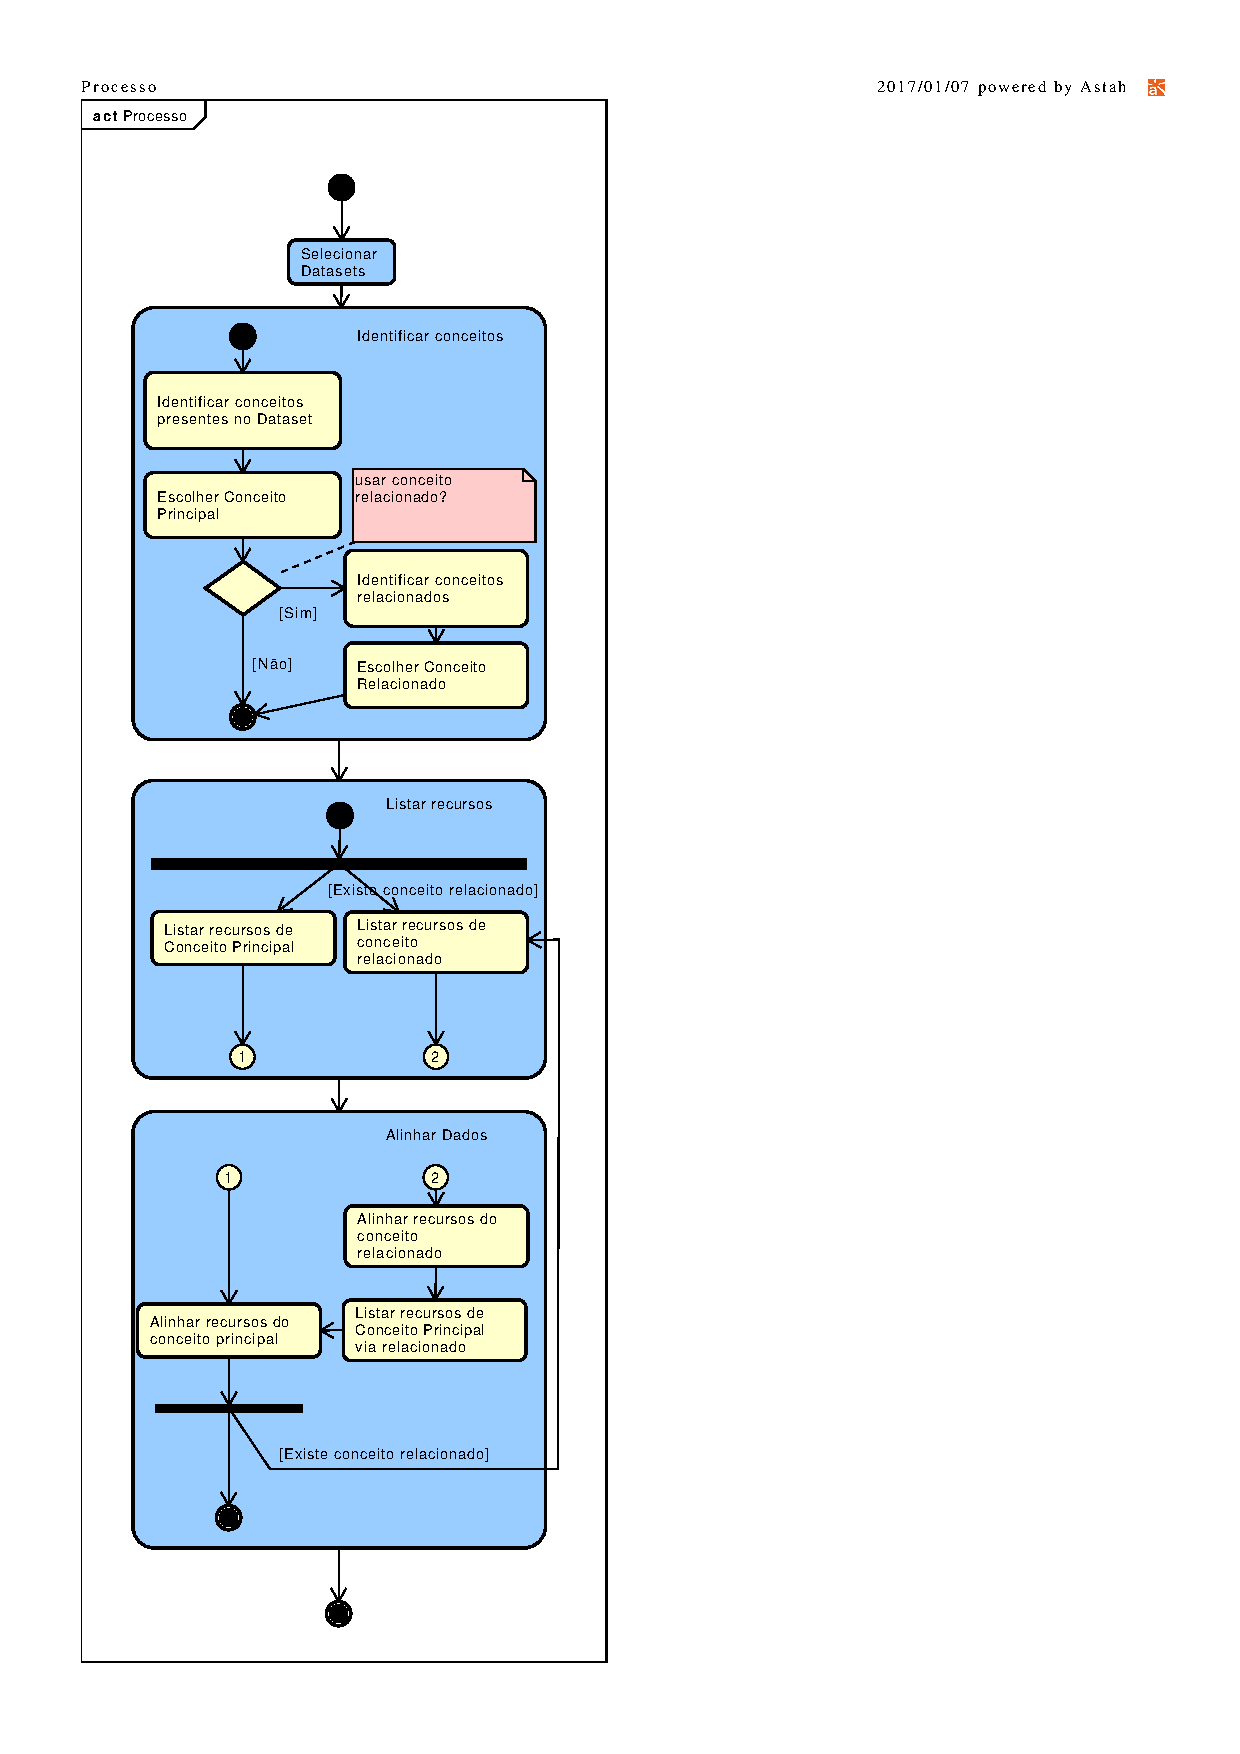
\includegraphics[width=0.9\textwidth]{./imagens/processo.png}
    \caption{Processo de alinhamento de dados conectados}
	\label{fig:processo}
\end{figure}

\section{I - Selecionar Datasets}
A etapa de selecionar \textit{datasets} trata da determinação de quais conjuntos de dados serão alinhados. A seleção de um \textit{dataset} está sujeita a alguns critérios, tais como: estar estruturado em triplas e utilizar conceitos modelados em ontologias/vocabulários. Tais critérios foram determinados de acordo com o escopo do processo, pois este está limitado à dados conectados. Além de se adequar ao escopo, os critérios cumprem os requisitos mínimos para a execução do processo.
Complementarmente, a comunidade já disponibiliza ferramentas e processos para a publicação de dados conectados na Web, o que não é o foco desse processo. Além disso, é importante destacar que ao modelar os dados em qualquer processo de publicação de dados conectados são utilizadas ontologias/vocabulários que podem servir como base.

\section{II - Identificar Conceitos}
Para auxiliar na escolha do conceito bem como os conceitos que estão relacionados foi desenvolvida duas consultas SPARQL. A primeira consulta explora a ontologia, principalmente as relações rdfs:domain e rdfs:range dos  as propriedades de objeto (ver código \ref{lst:sparql}). A segunda explora os dados e as relações estabelecidas pelas instâncias.
Na consulta \ref{lst:sparql}, a linha 4 tem o papel de recuperar todos os conceitos pertencentes na ontologia ou vocabulário. Na linha 5 é aplicada uma restrição. Nesta os conceitos devem ser domínio ou range de uma relação. Consequentemente, uma instância desse conceito será sujeito ou objeto de uma tripla (ver Figura \ref{fig:subgrafo1}).
\begin{figure}[!ht]
	\centering
	\includegraphics[width=0.9\textwidth]{./imagens/subgrafo_semantico.pdf}
	\caption{Relação entre ontologia e dados}
	\label{fig:subgrafo1}
\end{figure}

\begin{lstlisting}[captionpos=b, caption= Consulta SPARQL para identificação de conceito, label=lst:sparql,
basicstyle=\ttfamily,frame=single]
PREFIX rdf: <http://www.w3.org/1999/02/22-rdf-syntax-ns#>
PREFIX rdfs: <http://www.w3.org/2000/01/rdf-schema#>
select distinct ?Concept count(*) as ?count where {
[] 	a ?Concept.
?Concept 	(^rdfs:domain|^rdfs:range) ?o.
}
group 	by ?Concept	
order 	by desc(?count)
\end{lstlisting}

A consulta \ref{lst:sparql2} é comporta de duas partes, visto que o conceito pode modelar instâncias que são sujeito ou objeto de uma relação. Na primeira parte, o conceito selecionado representa o sujeito da tripla. Através das relações das instâncias é possível recuperar os conceitos que modelam as instâncias  relacionadas (objetos). Na segunda parte ocorre o inverso, o conceito representa o objeto da tripla e os conceitos que representam os sujeitos são recuperados.

\begin{lstlisting}[captionpos=b, caption=Query SPARQL para recuperação de conceitos relacionados, label=lst:sparql2,
   basicstyle=\ttfamily,frame=single]
PREFIX rdf: <http://www.w3.org/1999/02/22-rdf-syntax-ns#>
PREFIX rdfs: <http://www.w3.org/2000/01/rdf-schema#>


select distinct ?type where {
	values ?Concept{<URI do conceito escolhido>}
	{
		?instance rdf:type ?Concept; ?p ?o.
		?p rdf:type owl:ObjectProperty.
		?o rdf:type ?type.
	}
	union
	{
		?s ?p ?o.
		?p rdf:type owl:ObjectProperty.
		?o rdf:type ?Concept.
		?s rdf:type ?type.
	}
}

\end{lstlisting}

Como resultado do Código \ref{lst:sparql2} é provida uma lista contendo os conceitos relacionados ao conceito escolhido. Neste momento, o usuário deve escolher, quais conceitos relacionados ele deseja utilizar para melhorar o alinhamento do conceito escolhido. A escolha dos conceitos, assim como a quantidade de conceitos relacionados pode ser realizada de forma arbitrária. Essa decisão influenciará tanto no tempo que o processo levará para concluir, quanto na quantidade de recursos alinhados ao final do processo, pois para cada conceito relacionado haverá uma nova execução das etapas (iii) e (iv). Esse loop é necessário, pois alguns alinhamentos serão possíveis apenas através da relação entre esses conceitos.

\section{III - Listar recursos}
A etapa de listar recursos pode ser entendida como a recuperação dos recursos que pertencem aos conceitos. É importante destacar que a listagem/recuperação de recursos da base de conhecimento pode ser executada mais de uma vez durante o processo, gerando um conjunto de recursos para cada conceito escolhido. Além disso, essa etapa é responsável pela geração de pares candidatos, onde os recursos do \textit{Dataset} $D_{1}$ são comparados com os recursos do \textit{dataset} $D_{2}$.


\section{IV - Alinhar Dados}
A etapa de alinhamento de dados está dividida em duas atividades sendo elas: (i) alinhamento simples e (ii) alinhamento em cascata, que serão detalhadas nas subseções a seguir.

\subsection{alinhamento simples}
\label{im_simples}
Para alinhar os recursos é necessário executar alguns procedimentos, sendo eles o tratamento dos dados, comparação entre recursos e análise da similaridade. O primeiro procedimento se refere a transformações nas propriedades dos recursos. Essas transformações são necessárias para auxiliar os algoritmos de similaridade a analisar melhor a semelhança entre os recursos. No procedimento de comparação, cada uma da propriedades são analisadas. Caso uma propriedade não pertença a um dos recursos, ela é dispensada da comparação. A Figura  \ref{fig:resources} apresenta a comparação entre as propriedades de cada recurso.

\begin{figure}[!ht]
	\centering
	\includegraphics[width=0.6\textwidth]{./imagens/resources.png}
    \caption{Comparação entre recursos}
	\label{fig:resources}
\end{figure}

Para definir a similaridade entre as instâncias foram usadas duas equações. A Equação \ref{eq:properties_definition} define o conjunto de propriedades que será considerado durante a comparação entre os recursos, que será obtido a partir da diferença entre  o maior conjunto de propriedades e o conjunto de propriedades que deve ser desconsiderado. Logo:

\begin{equation}
P_f =M a x  ( P_{r1} ,P_{r2} ) - P_d
\label{eq:properties_definition}
\end{equation}

Onde:
\begin{itemize}
	\item $P_{r1}$ – Propriedades do recurso 1;
	\item $P_{r2}$ –  Propriedades do recurso 2;
	\item $P_d$ –  Propriedades que devem ser desconsideradas;
	\item $M a x  ( P_{r1} ,P_{r2} )$ – Retorna o maior conjunto de propriedades;
\end{itemize}

A Equação \ref{eq:similaridade} trata da função de similaridade entre recursos, essa equação pode ser entendida como a média das similaridades entre dois recursos.

\begin{equation}
SR  = \frac{1}{|P_f|} { \sum_{i = 1}^{P_f} {S(V(R_1,P_f[i]);V(R_2,P_f[i]))}}
\label{eq:similaridade}
\end{equation}

Onde:

\begin{itemize}
	\item S – Função de similaridade léxica;
	\item V(R,P) – Valor da propriedade P em um recurso R;
	\item $R_1$ – Recurso 1;
	\item $R_2$ – Recurso 2;
\end{itemize}

O valor gerado pelo componente de similaridade é enviado para o componente de alinhamento.

\subsection{Alinhamento em cascata}
\label{sub:cascata}
O alinhamento em cascata recebe esse nome devido as atividades que são executadas nesta etapa que são: Alinhamento simples dos recursos relacionados, Recuperação das instâncias que pertencem ao conceito principal que estão relacionadas aos recursos relacionados e alinhamento simples das instâncias recuperadas (ver Figura \ref{fig:cascata}).

\begin{figure}[!ht]
	\centering
	\includegraphics[width=0.6\textwidth]{./imagens/cascata.pdf}
	\caption{Alinhamento em cascata}
	\label{fig:cascata}
\end{figure}

\subsubsection{Alinhar Recursos}

Nesta atividade as instâncias que pertencem aos conceitos selecionados são alinhados. Para alinhar esses recursos é executado a etapa de alinhamento simples.

\subsubsection{Recuperar Recursos do conceito principal}
\label{recuperao}

A recuperação das instâncias que pertencem ao conceito principal é realizada a partir do  alinhamento dos recursos relacionados.A Figura \ref{fig:relacionados} representa abstratamente a construção dos pares candidatos a partir dos alinhamentos dos recursos relacionados.

\subsubsection{Alinhar Recursos Recuperados}

A partir das listas de candidatos geradas na atividade \ref{recuperao} o processo de alinhamento simples é executado.

\begin{figure}[!ht]
	\centering
	\includegraphics[width=0.8\textwidth]{./imagens/relacionados.pdf}
    \caption{Construção de pares candidatos a partir de recursos relacionados}
	\label{fig:relacionados}
\end{figure}